\documentclass[manuscript,screen,review, 12pt, nonacm]{acmart}
\let\Bbbk\relax % Fix for amssymb clash 
\usepackage{vmlmacros}
\AtBeginDocument{%
  \providecommand\BibTeX{{%
    \normalfont B\kern-0.5em{\scshape i\kern-0.25em b}\kern-0.8em\TeX}}}
\usepackage{outlines}
\setlength{\headheight}{14.0pt}
\setlength{\footskip}{13.3pt}
\title{An Alternative to Pattern Matching, Inspired by Verse}

\author{Roger Burtonpatel}
\email{roger.burtonpatel@tufts.edu}
\affiliation{%
\institution{Tufts University}
\streetaddress{419 Boston Ave}
  \city{Medford}
  \state{Massachusetts}
  \country{USA}
  \postcode{02155}
  }
\begin{document}
  

\section{\VMinus can be compiled to a decision tree}
\label{vminustod}
% [Evidence that \dots efficiency]
    Section~\ref{vcbadcost} claimed that pattern matching has a desirable
    efficiency property. More specifically, pattern matching can be compiled to
    a decision tree, which~~\citet{macqueen1985tree} built the foundation for in
    \it{Tree pattern matching for ML.} and~\citet{maranget} expanded on in his
    distinguished work, \it{Compiling Pattern Matching to Good Decision Trees}.
    To demonstrate that \VMinus has the same desirable cost model as pattern
    matching, I present an algorithm for compiling \VMinus to a decision tree.
    This algorithm runs during \DTran, the transformation from \VMinus to \D.
    Its domain, instead of a \it{case} expression, is \VMinus's \it{if-fi}. 
       
    \subsection{\D is a simple generalization of Maranget's trees} 

    % \rab{Do italics on italics cancel out in a cs paper as well? I un-italicized
    % D in this automatically-italicized subsection title; is that right?}

    Decision trees in \D are engineered to look like Maranget's trees. There
    are a few minor differences: First, Maranget's compilation algorithm is more
    complex than the one in this paper, and involves an intermediate
    representation of occurrence vectors and clause matrices which the algorithm
    I present does not use. Second, Maranget's trees are evaluated using a stack
    of values to scrutinize, while \D's trees are evaluated with internal
    environment of values. 

    The underlying structures of Maranget's and \D's decision trees, however,
    are analogous. The same operation is the heart of their evaluation: they
    take a value, examine it, and choose a branch based on its form (Maranget
    calls the operation \textsc{Switch}; we call it \it{test}). 

    Let's look at an example from \it{Compiling Pattern Matching to Good
    Decision Trees} which shows the structure of a simple pattern-matching
    function and its corresponding decision tree, then at a corresponding tree
    in \D. 

    Maranget beings with the function, \tt{merge}, which merges two lists: 

    \begin{figure}[H]
        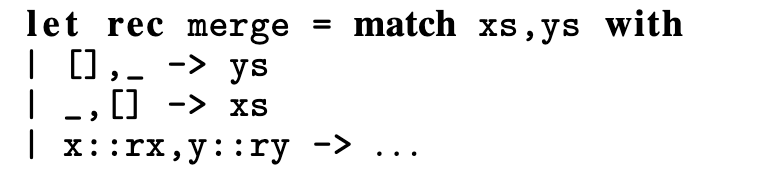
\includegraphics[scale=0.7]{../tex/images/merge.png}
        \Description{Maranget's merge implementation}
        \caption{The skeleton of Maranget's \tt{merge}}
    \end{figure}

    He then shows an intermediate representation in his compilation algorithm,
    the occurrence vector and clause matrix: 

    \begin{figure}[H]
        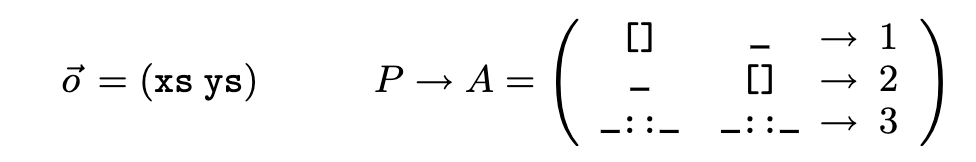
\includegraphics[scale=0.7]{../tex/images/occurence-and-matrix.png}
        \Description{Occurrence vector of names, and clause matrix of matches}
        \caption{The occurrence vector and clause matrix are intermediate
        representations in Maranget's compilation. I do not exploit this
        representation in my own algorithm, but it helps to understand his final
        tree.}
    \end{figure}

    Finally, he shows the final decision tree: 

    \begin{figure}[H]
        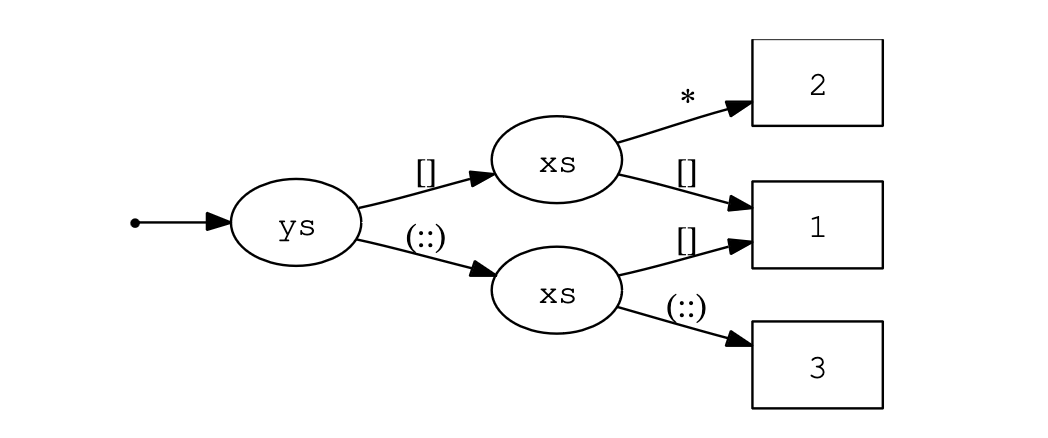
\includegraphics[scale=0.7]{../tex/images/dtree.png}
        \Description{The final decision tree for merge} 
        \caption{The final compiled decision tree for \tt{merge}, right-to-left}
    \end{figure}

    Here is the decision tree for \tt{merge} in \D. 

    \begin{figure}[H]
        \rab{This will be inserted when the match compiler is complete and we 
        know exactly what this tree looks like.}
        \Description{The decision tree for merge, now in D} 
        \caption{The tree for \tt{merge} in D looks \dots \rab{we'll know soon!}}
    \end{figure}


    \subsection{Rules (Big-step Operational Semantics) for \D:}
    
    \rab{Here is where the operational semantics for \D will live.}
    % \dsemantics

    \subsection{\D has a favorable cost model}
    I choose decision trees as a target for compilation for the simple reason of
    their appealing cost model. A decision tree can be exponential in size but
    never examines a word of the scrutinee more than once. It is the compilation
    from \VMinus to \D that must enforce this invariant by determining which
    equations in an \it{if-fi} represent “decision points” and compiling them to
    unique \it{test} nodes in the resulting tree. 
    
    \subsection{The \DTran\ algorithm: \VMinus $\rightarrow$ \D}

    Before presenting the algorithm \DTran, I will explain in plain English how
    it works, with a bit of hand-waving. The algorithm is non-trivial, so my
    hope is that the English answers any questions you may have after reading 
    the formalism. 

    When presented with an \it{if-fi}, \DTran\ introduces all the names under
    the all existential $\exists$'s to a context which determines if a name is
    \it{known} or \it{unknown}. At the start, each name introduced by $\exists$
    is \it{unknown}. Since all names are unique at this stage, there are no
    clashes. 


    \rab{I describe the algorithm in plain English here.}

    % \DTran\ then repeatedly chooses a guarded expression $G$ and attempts the
    % following: 

    % \begin{enumerate}
    %     \item If there are no guards, insert a \it{match} node with the
    %     right-hand side of $G$. 
    %     \item Choose an equation in $G$ of the form $x = K \dots$ s.t. $x$ is
    %     \it{known}. 
    %     \item If one is found, use it to generate a \it{test} node, building
    %     each subtree of the \it{test} by pruning all branches in \it{all}
    %     guarded expressions of the \it{if-fi} in which $x = e$ and $e \neq K
    %     \dots$ and invoking \DTran\ on the remaining ones with a context where
    %     $x$ is known. The algorithm builds the default tree of the \it{test} by
    %     finding it in the \it{if-fi} or assembling one that fails at runtime. 
    %     \item If no equation of the form \it{x = K \dots} is found, try to 
    %     find a condition $e$ s.t. all names in $e$ are known. 
    %     \item If one is found, use it to generate a \it{let}-\it{if-then-else}
    %     pair, pruning each subtree of $e$. 
    %     \item If no condition $e$ is found, try to find an equation $x = e$ s.t.
    %     both $x$ and all names in $e$ are \it{known}.
    %     \item If one is found, generate a \it{let} node, make $x$ known, prune
    %     the \it{if-fi} of all duplicate instances of that $x = e$, and invoke
    %     \DTran\ again. 
    %     \item If none is found, the \it{if-fi} cannot be compiled to a decision
    %     tree. The algorithm halts with an error. 
    % \end{enumerate}

    The algorithm terminates when inserts a final \it{match} node for a
    right-hand side expression $e$ when the list of guards preceding $e$ is
    empty or a list of assignments from names to unbound names. Termination of
    \DTran\ is guaranteed because each recursive call passes a list of guarded
    expressions in which the number of guards is strictly smaller, so eventually
    the algorithm reaches a state in which the first unmatched branch is all
    trivially-satisfied guards. 

    % \DTran\ makes the distinction for an equation \it{x = e}
    % based off of this model: 
    % \begin{enumerate}
    % \item 
    % \end{enumerate}
    % No guards  ==  MATCH
    % CONDITION  ==   if known, convert to LET, IF
    % EQN (x, e) ==
    %    - if x is known and e is VCONAPP, generate TEST
    %    - if x is known and e is not VCONAPP and e is known
    %         generate LET, IF
    %    - if x is unknown and e is known, then generate LET
       
%  What if we don't find any of the above? 
%  There must be only unknown guards. 
%  Can't compile! 
    
    % For an equation that
    % represents a binding of values to values, the algorithm inserts a \it{let}
    % node, and for a condition guard \it{e}, it inserts a \it{let} followed by 
    % an \it{if-then-else}. 
    
    
    
    \rab{Here will live the formal algorithm for \DTran}.

    \subsection{Translation from \VMinus to \D preserves semantics}
    
    Translating \it{if-fi} to a decision tree should preserve semantics. The
    following theorem formalizes this claim: 

    \rab{Here will live the theorem of semantics preservation}. 
    
    \begin{proof}
        See appendix A. 
    \end{proof}
    % \2 \bf{Likely inductive hypothesis. 1-4 sentences on proof max. }

\end{document}